\documentclass[a4paper,12pt]{article}
\usepackage[fontset=none]{ctex}
\usepackage{fancyhdr}
\usepackage{wrapfig}

% 数学公式和化学方程式
\usepackage{amsmath, amsthm, amssymb, amsfonts}
\usepackage{latexsym,bm}
\usepackage[version=4]{mhchem}
\makeatletter
\newcommand{\rmnum}[1]{\romannumeral #1}%小写罗马数字
\newcommand{\Rmnum}[1]{\expandafter\@slowromancap\romannumeral #1@}%大写罗马数字
\makeatother
\renewcommand{\frac}{\dfrac}
\renewcommand{\leq}{\leqslant}
\renewcommand{\geq}{\geqslant}
\renewcommand{\le}{\leqslant}
\renewcommand{\ge}{\geqslant}
\renewcommand{\epsilon}{\varepsilon}

\newcommand{\tran}{^T}
\newcommand{\conj}[1]{{\overline{#1}}}
\newcommand{\hermconj}{^H}

\newcommand{\va}{{\bm{a}}}
\newcommand{\vb}{{\bm{b}}}
\newcommand{\vc}{{\bm{c}}}
\newcommand{\vd}{{\bm{d}}}
\newcommand{\ve}{{\bm{e}}}
\newcommand{\vf}{{\bm{f}}}
\newcommand{\vg}{{\bm{g}}}
\newcommand{\vh}{{\bm{h}}}
\newcommand{\vi}{{\bm{i}}}
\newcommand{\vj}{{\bm{j}}}
\newcommand{\vk}{{\bm{k}}}
\newcommand{\vl}{{\bm{l}}}
\newcommand{\vm}{{\bm{m}}}
\newcommand{\vn}{{\bm{n}}}
\newcommand{\vo}{{\bm{o}}}
\newcommand{\vp}{{\bm{p}}}
\newcommand{\vq}{{\bm{q}}}
\newcommand{\vr}{{\bm{r}}}
\newcommand{\vs}{{\bm{s}}}
\newcommand{\vt}{{\bm{t}}}
\newcommand{\vu}{{\bm{u}}}
\newcommand{\vv}{{\bm{v}}}
\newcommand{\vw}{{\bm{w}}}
\newcommand{\vx}{{\bm{x}}}
\newcommand{\vy}{{\bm{y}}}
\newcommand{\vz}{{\bm{z}}}
\newcommand{\vzero}{{\bm{0}}}

\newcommand{\vepsilon}{{\bm{\epsilon}}}
\newcommand{\vtheta}{{\bm{\theta}}}
\newcommand{\vpsi}{{\bm{\psi}}}
\newcommand{\vpi}{{\bm{\pi}}}
\newcommand{\vphi}{{\bm{\phi}}}

\newcommand\bigO{{\mathcal{O}}}

\newcommand{\vA}{{\bm{A}}}
\newcommand{\vB}{{\bm{B}}}
\newcommand{\vC}{{\bm{C}}}
\newcommand{\vD}{{\bm{D}}}
\newcommand{\vE}{{\bm{E}}}
\newcommand{\vF}{{\bm{F}}}
\newcommand{\vG}{{\bm{G}}}
\newcommand{\vH}{{\bm{H}}}
\newcommand{\vI}{{\bm{I}}}
\newcommand{\vJ}{{\bm{J}}}
\newcommand{\vK}{{\bm{K}}}
\newcommand{\vL}{{\bm{L}}}
\newcommand{\vM}{{\bm{M}}}
\newcommand{\vN}{{\bm{N}}}
\newcommand{\vO}{{\bm{O}}}
\newcommand{\vP}{{\bm{P}}}
\newcommand{\vQ}{{\bm{Q}}}
\newcommand{\vR}{{\bm{R}}}
\newcommand{\vS}{{\bm{S}}}
\newcommand{\vT}{{\bm{T}}}
\newcommand{\vU}{{\bm{U}}}
\newcommand{\vV}{{\bm{V}}}
\newcommand{\vW}{{\bm{W}}}
\newcommand{\vX}{{\bm{X}}}
\newcommand{\vY}{{\bm{Y}}}
\newcommand{\vZ}{{\bm{Z}}}

\newcommand{\ones}[1]{{\bm{1}_{#1}}}
\newcommand{\zeros}[1]{{\bm{0}_{#1}}}
\newcommand{\eye}[1]{{\bm{E}_{#1}}}

\newcommand{\vect}[1]{{\bm{#1}}}
\newcommand{\mat}[1]{{\bm{#1}}}

\renewcommand{\d}{{\mathrm{d}}}
\newcommand{\pder}[2]{{\frac{\partial #1}{\partial #2}}}
\newcommand{\oder}[2]{{\frac{\mathrm{d} #1}{\mathrm{d} #2}}}
\newcommand{\npder}[2]{{\nicefrac{\partial #1}{\partial #2}}}
\newcommand{\popt}[2]{{\frac{\partial}{\partial #2}#1}}
\newcommand{\oopt}[2]{{\frac{\mathrm{d}}{\mathrm{d} #2}#1}}
\newcommand{\inte}[4]{{\int_{#1}^{#2}#3\mathrm{d}#4}}

\newcommand{\argmin}{{\operatornamewithlimits{argmin}}}
\newcommand{\argmax}{{\operatornamewithlimits{argmax}}}
\newcommand{\tr}{{\mathrm{tr}}}
\newcommand{\Prob}{{\mathrm{P}}}
\newcommand{\E}{{\mathrm{E}}}
\newcommand{\D}{{\mathrm{D}}}

\newcommand{\<}{{\langle}}
\renewcommand{\>}{{\rangle}}



% 插入PDF文件
\usepackage[final]{pdfpages}

% 引文使用
\usepackage[backend=biber,style=gb7714-2015,gbpub=false]
{biblatex}%align=gb7714-2015
\addbibresource[location=local]{Ref/Collection.bib}
% \usepackage[colorlinks=true,pdfstartview=FitH,%
% linkcolor=blue,anchorcolor=violet,citecolor=magenta]{hyperref}%加载hyperref宏包,使用超链接

% 插图使用
\usepackage{graphicx}
\usepackage{float}
% \usepackage{epstopdf}
\usepackage{caption}
\usepackage{subfigure}  %插入多图时用子图显示的宏包

% 表格使用
\usepackage{bigstrut}
\usepackage{booktabs}
\usepackage{multicol}
\usepackage{multirow}

% LaTeX距离设置:
% mm	毫米	1 mm = 2.845 pt
% pt	点		1 pt = 0.351 mm
% bp	大点	1 bp = 0.353 mm > 1 pt
% dd	迪多	1 dd = 0.376 mm = 1.07 pt
% pc	排卡	1 pc = 4.218 mm = 12 pt
% sp	定标点	65536 sp = 1 pt
% cm	厘米	1 cm= 10 mm= 28.453 pt
% cc	西塞罗	1 cc= 4.513 mm= 12 dd = 12.84 pt
% in	英寸	1 in = 25.4 mm = 72.27 pt
% ex	ex	1 ex = 当前字体尺寸中 x 的高度
% em	em	1 em = 当前字体尺寸中 M 的宽度

% 字体大小:
\newcommand{\chuhao}{\fontsize{42.2pt}{\baselineskip}\selectfont}
\newcommand{\xiaochu}{\fontsize{36.1pt}{\baselineskip}\selectfont}
\newcommand{\yihao}{\fontsize{26.1pt}{\baselineskip}\selectfont}
\newcommand{\xiaoyi}{\fontsize{24.1pt}{\baselineskip}\selectfont}
\newcommand{\erhao}{\fontsize{22.1pt}{\baselineskip}\selectfont}
\newcommand{\xiaoer}{\fontsize{18.1pt}{\baselineskip}\selectfont}
\newcommand{\sanhao}{\fontsize{16.1pt}{\baselineskip}\selectfont}
\newcommand{\xiaosan}{\fontsize{15.1pt}{\baselineskip}\selectfont}
\newcommand{\sihao}{\fontsize{14.1pt}{\baselineskip}\selectfont}
\newcommand{\xiaosi}{\fontsize{12.1pt}{\baselineskip}\selectfont}
\newcommand{\wuhao}{\fontsize{10.5pt}{\baselineskip}\selectfont}
\newcommand{\xiaowu}{\fontsize{9.0pt}{\baselineskip}\selectfont}
\newcommand{\liuhao}{\fontsize{7.5pt}{\baselineskip}\selectfont}
\newcommand{\xiaoliu}{\fontsize{6.5pt}{\baselineskip}\selectfont}
\newcommand{\qihao}{\fontsize{5.5pt}{\baselineskip}\selectfont}
\newcommand{\bahao}{\fontsize{5pt}{\baselineskip}\selectfont}

% 字体
% \usepackage{fontspec, xunicode, xltxtra}
% \usepackage{xeCJK}
\setmainfont{Times New Roman}
\setsansfont{Droid Sans}
\setmonofont{Courier New}
\setCJKmainfont[Path="Style/",AutoFakeBold,ItalicFont=simkai.ttf]{simsun.ttc}
\setCJKsansfont[Path="Style/",AutoFakeBold]{simhei.ttf}
\setCJKmonofont[Path="Style/",AutoFakeBold]{simfang.ttf}
% 需要的话
%\setCJKfamilyfont{zhfs}[AutoFakeBold]{simfang.ttc}
%\setCJKfamilyfont{zhkai}[AutoFakeBold]{simkai.ttf}
%\setCJKfamilyfont{zhsong}[AutoFakeBold]{simsun.ttc}
\setCJKfamilyfont{zhhei}[AutoFakeBold]{simhei.ttf}

\newcommand{\heiti}{\CJKfamily{zhhei}}


\usepackage{titlesec}
%section等前后间距
\titlespacing*{\section}{0pt}{1ex plus .0ex minus .0ex}{1ex plus .0ex}
\titlespacing*{\subsection}{0pt}{0ex plus .0ex minus .0ex}{0ex plus .0ex}
%section等字体设置和字号大小
\titleformat*{\section}{\large\bfseries}
\titleformat*{\subsection}{\normalsize\bfseries}

%纸张和页边距
\usepackage[a4paper,left=1.5cm,right=1.5cm,top=1.5cm,bottom=1.5cm]{geometry}

%行间距
\usepackage{setspace}
\renewcommand{\baselinestretch}{1.5}
\AtBeginDocument{
    \setlength{\abovedisplayskip}{1.5pt}%公式前后间距,强行在导言区中设置
    \setlength{\belowdisplayskip}{1.5pt}%
    \setlength{\abovedisplayshortskip}{1.5pt}%
    \setlength{\belowdisplayshortskip}{1.5pt}%
    %图片和浮动对象间距
    \setlength{\floatsep}{2pt plus 2pt minus 2pt}%出现在页面的顶部或底部的浮动对象之间的垂直距离。 缺省为 12pt plus 2pt minus 2pt
    \setlength{\textfloatsep}{2pt plus 2pt minus 2pt}%出现在页面的顶部或底部的浮动对象与文本之间的垂直距离。缺省为 20pt plus 2pt minus 4pt
    \setlength{\intextsep}{2pt plus 2pt minus 2pt}%出现在页面中间的浮动对象(如使用了 h 选项 的浮动对象)与上下方文本之间的垂直距离。 缺省为 12pt plus 2pt minus 2pt
}
% 间距有关变量:
% \baselineskip:行基线间距。
% \lineskip:行间距。
% \baselinestretch:伸展因子。
% \parskip:部分段间距。
% \lineskiplimit:当两行字之间的距离小于\lineskiplimit时,行距自动设为\lineskip。
% 段间距:\lineskip + \parskip
% 行间距:\lineskip = \baselineskip * \baselinestretch

%首行缩进
\usepackage{indentfirst}
\setlength{\parindent}{2pt}

%文本和图片等浮动对象占比
\renewcommand{\floatpagefraction}{.85}%浮动页中浮动对象最大占比
\renewcommand{\textfraction}{.15}%文本页中文本最小占比
\renewcommand{\topfraction}{.65}%页面顶部可以用来放置浮动对象的高度与整个页面高度的最大比例
\renewcommand{\bottomfraction}{.60}

%符号列表间距设置
% \setlength{\leftmargin}{1.2em}%左边界
% \setlength{\parsep}{0ex}%段落间距
% \setlength{\topsep}{1ex}%列表到上下文的垂直距离
% \setlength{\itemsep}{0.5ex}%条目间距
% \setlength{\labelsep}{0.3em}%标号和列表项之间的距离,默认0.5em
% \setlength{\itemindent}{1.1em}%标签缩进量
% \setlength{\listparindent}{0em} %段落缩进量

% 列表格式
\usepackage{enumitem}
\setenumerate{itemsep=0pt,partopsep=0pt,parsep=\parskip,topsep=5pt,itemindent=2em}
\setitemize{itemsep=0pt,partopsep=0pt,parsep=\parskip,topsep=5pt,itemindent=2em}
\setdescription{itemsep=0pt,partopsep=0pt,parsep=\parskip,topsep=5pt,itemindent=2em}

% 页码设置
\pagestyle{empty}

% 水印
\usepackage{eso-pic}
\newcommand\BackgroundPicture{%
  \put(0,0){%
    \parbox[b][\paperheight]{\paperwidth}{%
      \vfill
      \centering%
\begin{tikzpicture}[remember picture,overlay]
\node [rotate=45,scale=6,text opacity=0.3] at (current page.center) {水印样例}; %中括号内是旋转角度,字体大小
\end{tikzpicture}%
      \vfill
    }}}

% 标题样式
\newcommand\subtitle[1]{{\Large #1}} % 定义副标题
\makeatletter % change default title style
\renewcommand*\maketitle{%
    \begin{center}% 居中标题
        % \bfseries % 默认粗体
        {\LARGE\bfseries\@title \par} % LARGE字号,默认粗体
        \vskip 1em% %%%  标题下面只有1em的缩进或margin
        {\@author \par}
        % {\global\let\author\@empty}%
        {\global\let\date\@empty}%
        \thispagestyle{empty} %  不设置页面样式
    \end{center}%
  \setcounter{footnote}{0}%
}
\makeatother

% 中文摘要
\newenvironment{cnabstract}{%
  \par\sihao
  \noindent\mbox{}\hfill{\bfseries\textsf \cnabstractname}\hfill\mbox{}\par
  \vskip 2.5ex}{\par\vskip 2.5ex}
\newcommand{\cnabstractname}{摘 要}

% 页眉页脚
\pagestyle{fancy}
\fancypagestyle{preContent}{
    \fancyhead{}
    \renewcommand\headrulewidth{0pt}
    \fancyfoot[C]{\thepage}
}

% 插入代码设置
\usepackage{listings}
\lstset{
 columns=fixed,       
 numbers=left,                                        % 在左侧显示行号
 numberstyle=\tiny\color{gray},                       % 设定行号格式
 frame=none,                                          % 不显示背景边框
 backgroundcolor=\color[RGB]{245,245,244},            % 设定背景颜色
 keywordstyle=\color[RGB]{40,40,255},                 % 设定关键字颜色
 numberstyle=\footnotesize\color{darkgray},           
 commentstyle=\rmfamily\it\color[RGB]{0,96,96},                % 设置代码注释的格式
 stringstyle=\rmfamily\slshape\color[RGB]{128,0,0},   % 设置字符串格式
 showstringspaces=false,                              % 不显示字符串中的空格
 language=Python,                                        % 设置语言
 breaklines      =   true,
}

\begin{document}
\title{数据挖掘第一次上机实验报告}
\author{刘臻劼}

\begin{titlepage}
%本页为自定义的封面
	% \title{作业标题}
	% \author{作者}
	\newcommand{\ID}{{\Large 000000000}}
	\newcommand{\supervisor}{{\Large 李田所}}
	\newcommand{\class}{{\Large 班级}}
    
	\center
	\quad\\[1cm]
	
\includegraphics[width=12cm]{Content/西安电子科技大学-logo.jpg}\\[2cm]
	
	\quad\\[1cm]
	\makeatletter
	
	{\linespread{4}\Huge\bfseries\@title}\\[1cm]
	\begin{table}[H]
		\centering
		\subtitle{\textsf {基于图论与矩阵分解的协同过滤推荐方法对比}}\\[2.5cm]
		  \begin{tabular}{rl}
			{\Large 姓名:}&{\Large 刘臻劼}\\[0.5cm]
			{\Large 学号:}&{\Large 19030700016}\\[0.5cm]
			{\Large 班级:}&{\Large 1903071}\\[0.5cm]
			{\Large 导师:}&{\Large 郭杏莉}
		  \end{tabular}\\
	\end{table}
	\makeatother
	\quad\\[1cm]
	\vfill 
\end{titlepage} % 这个是封面,不需要刻意注释掉

\clearpage
\tableofcontents
\pagestyle{preContent}

\clearpage
\section{实验内容}
\subsection{实验目标}
\xiaosi\begin{spacing}{1.5} 本次实验目标为:在MovieLens数据集上构建“用户——电影”评分矩阵,基于评分矩阵对用户与电影进行推荐。
\end{spacing}
\subsection{数据集介绍}
\xiaosi\begin{spacing}{1.5}
MovieLens数据集包含6040个用户关于3883部电影的1000209条评分信息。数据集分为三个文件:用户数据users.dat、电影数据movies.dat和评分数据ratings.dat。\par
(1)用户数据\par
关于6040个用户的个人脱敏数据,格式为
{\setlength\abovedisplayskip{1pt}
\setlength\belowdisplayskip{1pt}
\begin{align}
UserID::Gender::Age::Occupation::Zip-code
\nonumber\end{align}
}
其中:\par
$UserID$:1到6040顺序编号;\par
$Gender$:F为女性,M为男性;\par
$Age$:分为1,18,25,35,45,50,56共7类,代表用户所属的年龄段;\par
$Occupation$:0到20的整数,分别代表21种职业;\par
$Zip-code$:邮编。\par
(2)电影数据\par
关于3883部电影的信息,格式为
{\setlength\abovedisplayskip{1pt}
\setlength\belowdisplayskip{1pt}
\begin{align}
MovieID::Title::Genres
\nonumber\end{align}
}
其中:\par
$MovieID$:1到3952无重复的整数,非连续编号;\par
$Title$:电影名,为电影名与年份的拼接,如“Toy Story (1995)”;\par
$Genres$:电影所属的类别,如果同属多个类别,则类名间用“|”隔开,如:“Adventure|Children's”。\par
(3)评分数据\par
用户对电影的1000209条评分数据,格式为
{\setlength\abovedisplayskip{1pt}
\setlength\belowdisplayskip{1pt}
\begin{align}
UserID::MovieID::Rating::Timestamp
\nonumber\end{align}
}
其中:\par
$UserID,\ MovieID$:同上;\par
$Rating$:1到5之间(含)的整数;\par
$Timestamp$:自1970年1月1日零点后到用户提交评价的时间的秒数。
\end{spacing}


\clearpage
\section{实验分析}
\subsection{题目分析}
\xiaosi\begin{spacing}{1.5}
原问题包含两个要求,一是对题给的用户——电影打分数据集进行建模。再是完善评分矩阵并进行推荐。\par
\begin{wrapfigure}{r}{5cm}%靠文字内容的右侧
\centering
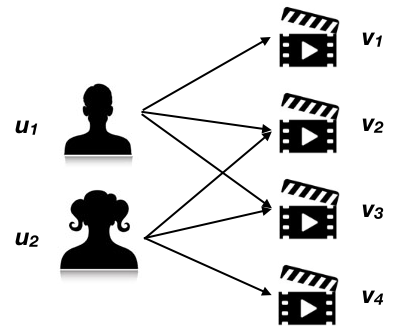
\includegraphics[width=0.27\textwidth]{Figure/simrank-f1.png}
\caption{二部图模型}
\end{wrapfigure}
(1)用户——电影打分建模\par
我们考虑用户集 $U=\{u_1,u_2,\cdots u_n\},n=6040$,电影集 $V=\{v_1,v_2,\cdots,v_m\},m=3883$。则用户对电影的评分可视作以 $U,\ V$ 构建的二部图 $G=<U,V,E>$ 相应边的权重,其中边集 $E \subseteq U \times V$,则第$i$个用户对第$j$部电影的评分 $r_{ij}=h(u_i,v_j),\ h:E\rightarrow [0,5]$,此处评分函数的值域为$[0,5]$,将原始任务中的多类分类问题转化为了回归问题,这是考虑到评分允许浮点更加自然。\par
(2)评分矩阵\par
在(1)我们知道边集 $E \subseteq U \times V$,而实际上 $|E|\ll |U|\cdot|V|$,这说明全体用户对所有电影的评价矩阵 $\mathbf{R}=(r_{ij})_{m\times n}$ 是较稀疏的。而本实验的核心问题则是如何通过现有数据补全评价矩阵$\mathbf{R}$。补全评分矩阵后我们将基于此进行推荐。
\end{spacing}

\subsection{推荐算法简介}
\subsubsection{推荐算法的分类}
\xiaosi\begin{spacing}{1.5}
所谓推荐算法,即是根据用户行为推测其喜好的一类算法。推荐算法历史悠久,在机器学习还没有兴起的时候就有需求和应用了。概括来说,可以分为以下5种\cite{1}:\par
(1)基于内容的推荐:这一类一般依赖于NLP方法,通过挖掘文本的TF-IDF特征向量,来得到用户的偏好,进而做推荐。\par
(2)协调过滤推荐:协调过滤是推荐算法中目前最主流的种类,花样繁多,目前绝大多数实际应用的推荐算法都是协同过滤推荐算法。\par
(3)混合推荐:类似机器学习中的集成学习,博才众长,通过多个推荐算法的结合,得到一个更好的推荐算法。\par
(4)基于规则的推荐:这类算法常见的比如基于最多用户点击,最多用户浏览等,属于大众型的推荐方法,在目前的大数据时代并不主流。\par
(5)基于知识的推荐:在某种程度是可以看成是一种推理技术,它不是建立在用户需要和偏好基础上推荐的。\par
\end{spacing}
\subsubsection{协同过滤推荐算法}
\xiaosi\begin{spacing}{1.5}
我们接下来重点讨论协同过滤的推荐算法。协同过滤分析用户兴趣,在用户群中找到指定用户的相似(兴趣)用户,综合这些相似用户对某一信息的评价,形成对该指定用户对此信息的喜好程度预测。\par
协同过滤问题一般这样呈现:只有部分用户和部分对象之间是有评分数据的,其它部分评分是空白,此时我们要用已有的部分稀疏数据来预测那些空白的物品和数据之间的评分关系,找到最高评分的物品推荐给用户。很明显本实验属于一协同过滤问题。
\end{spacing}

\subsection{模型设计}
\xiaosi\begin{spacing}{1.5}
明确题意后,我们来讨论解决方法。针对本题考虑使用基于图论的方法与基于矩阵分解及深度学习方法。
\subsubsection{图论方法}
由 2.1 节,我们将用户——电影建模为二部图,我们可以考虑使用基于图的 SimRank \cite{2}算法。其核心思想是\cite{3}:如果两个用户相似,则与这两个用户相关联的物品也类似;如果两个物品类似,则与这两个物品相关联的用户也类似。
\subsubsection{矩阵分解结合深度学习}
协同过滤中另一经典算法为矩阵分解。我们希望评分矩阵有如下分解: 
{\setlength\abovedisplayskip{1pt}
\setlength\belowdisplayskip{1pt}
\begin{align}
\mathbf{R}_{m\times n}=\mathbf{P}_{m\times k}\mathbf{Q}_{k\times n}
\end{align}
}
而在此处我们不使用传统矩阵分解方法来求解矩阵 $\mathbf{P}$ 与 $\mathbf{Q}$,而是通过深度学习方法得到。\par
传统方法以及上文提到的图论方法仅利用了用户对电影的评分数据,其他诸如用户性别,电影名及类别等等信息则没有利用。通过深度学习方法可以更充分地利用全部信息。对于式(1),我们可以认为 $\mathbf{P}$ 为用户特征矩阵,$\mathbf{Q}$ 为电影特征矩阵。\par
(1)模型概览
模型的概览图如下:
\clearpage
\begin{figure}
\setlength{\abovecaptionskip}{0.cm}
\setlength{\belowcaptionskip}{-0.cm}
\centering
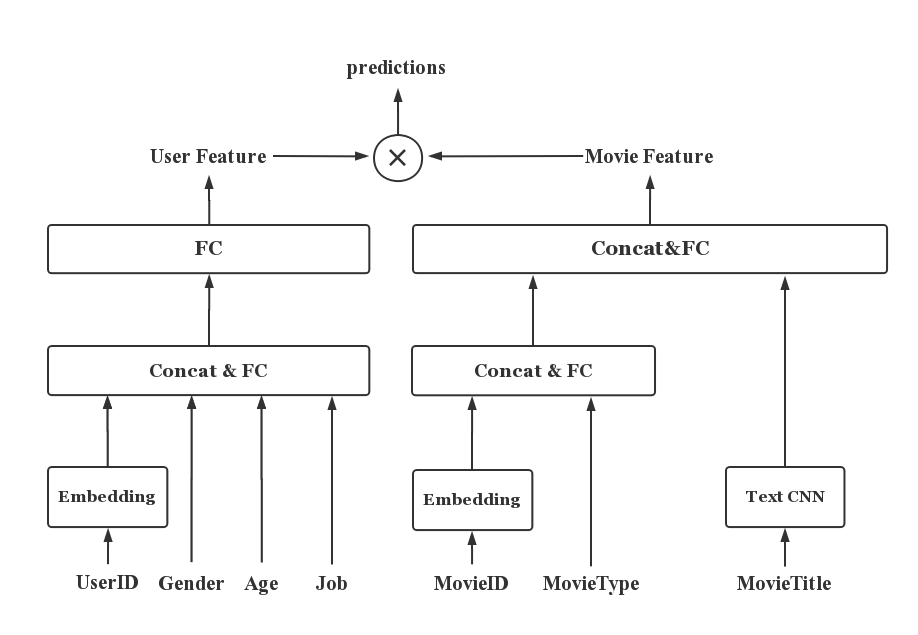
\includegraphics[width=0.8\textwidth]{Figure/2.png}
\caption{模型示意图}
\end{figure}

\par

(2)用户特征提取\par
用户信息中,对于 $Gender,\ Age,\ Job$ 三个字段的信息,由于类别数较少可以采用 One-Hot 编码。而 $UserID$ 由于类别太多故而此处采用Embedding方法,用$embedding\_ dim=32$ 维向量表示用户的ID值。\par
将 $UserID$ 的Embedding向量与其他信息One-Hot向量拼接并通过全连接层并通过 ReLU激活,而后再次通过全连接层并进行批归一化。至此得到了用户信息的特征矩阵。\par
(3)电影特征提取\par
对于电影信息中 $MovieID$ 与 $MovieType$ 字段,类似用户信息的处理。ID通过Embedding得到,电影类型为Multi-Hot向量。\par
而对于电影名称,此处采用CNN提取特征。CNN在NLP的应用最早来源于Kim在2014年的工作\cite{4}。相比CV领域,TextCNN结构较为简单,一般仅有词嵌入、卷积、池化与全连接四部分。而本文用其提取电影文本特征,仅包含词嵌入、卷积与池化三个部分。最后再将电影名称信息与电影信息拼接通过全连接层,得到电影信息的特征矩阵。\par
(4)拟合评分
上述步骤完成后,我们得到了用户特征矩阵 $\mathbf{P}_i \in \mathbb{R}^{batch\_ size \times hidden\_ size}$ 与电影特征矩阵 $\mathbf{Q}_i \in \mathbb{R}^{batch\_ size \times hidden\_ size}$,其中 $i$ 为批次数。则我们可以将二者逐点相乘,再按行求和作为模型拟合结果。通过计算与目标值的MSE误差得到梯度并反向传播优化。

\end{spacing}



\clearpage


\printbibliography%[heading=bibliography,title=参考文献]
\end{document}